% !TeX spellcheck = en_US 
\documentclass[12pt,english]{report}
\usepackage{tesi}
% CORSO DI LAUREA:
\def\myCDL{Master in\\Computer Science}

% TITOLO REPORT:
\def\myTitle{Algorithms for massive datasets \\
\large{Final report about Recommender System}}

% AUTORE:
\def\myName{Samuele Simone}
\def\myMat{Matr. Nr. 11910A}

\def\myRefereeA{Prof. Dario Malchiodi}

% ANNO ACCADEMICO
\def\myYY{2022-2023}

% Il seguente comando introduce un elenco delle figure dopo l'indice (facoltativo)
%\figurespagetrue

% Il seguente comando introduce un elenco delle tabelle dopo l'indice (facoltativo)
%\tablespagetrue


% Package di formato
\usepackage[a4paper]{geometry}		% Formato del foglio
\usepackage[english]{babel}			% Supporto per l'italiano
\usepackage[utf8]{inputenc}			% Supporto per UTF-8
%\usepackage[a-1b]{pdfx}			% File conforme allo standard PDF-A (obbligatorio per la consegna)

% Package per la grafica
\usepackage{graphicx}				% Funzioni avanzate per le immagini
\usepackage{hologo}					% Bibtex logo with \hologo{BibTeX}
%\usepackage{epsfig}				% Permette immagini in EPS
\usepackage{listings}
\usepackage{xcolor}
\usepackage{hyperref}

%Creating dark code theme for listings
\definecolor{codegreen}{rgb}{0.58,0.88,0.58}
\definecolor{codegray}{rgb}{0.5,0.5,0.5}
\definecolor{codeorange}{rgb}{0.72,0.54,0.45}
\definecolor{backcolour}{rgb}{0.10,0.13,0.14}
\definecolor{keyw}{rgb}{0.60,0.85,0.98}
\lstdefinestyle{mystyle}{
    backgroundcolor=\color{backcolour},   
    commentstyle=\color{codegreen},
    keywordstyle=\color{keyw},
    numberstyle=\tiny\color{codegray},
    stringstyle=\color{codeorange},
    basicstyle=\ttfamily\footnotesize \color{white},
    breakatwhitespace=false,         
    breaklines=true,                 
    captionpos=b,                    
    keepspaces=true,                 
    numbers=left,                    
    numbersep=5pt,                  
    showspaces=false,                
    showstringspaces=false,
    showtabs=false,                  
    tabsize=2
}

\lstset{style=mystyle}

% Package tipografici
\usepackage{amssymb,amsmath,amsthm} % Simboli matematici
\usepackage{listings}				% Scrittura di codice

% Package ipertesto
\usepackage{url}					% Visualizza e rendere interattii gli URL
\usepackage{hyperref}				% Rende interattivi i collegamenti interni
\usepackage{notes2bib}

\usepackage{multirow}
\hypersetup{
    colorlinks=true,
    linkcolor=blue,
    urlcolor=cyan,
    filecolor=magenta,  
    }
\begin{document}
% Creazione automatica del frontespizio
\frontespizio
{\raggedleft \large \sl \textit{I/We declare that this material, which I/We now submit for assessment, is entirely my/our own work and has not been taken from the work of others, save and to the extent that such work has been cited and acknowledged within the text of my/our work. I/We understand that plagiarism, collusion, and copying are grave and serious offences in the university and accept the penalties that would be imposed should I engage in plagiarism, collusion or copying. This assignment, or any part of it, has not been previously submitted by me/us or any other person for assessment on this or any other course of study.} \\}


\afterpreface

This report is made up of 8 chapters. In the \textbf{Chapter~\ref{ch:introduction}} we give at the reader a general view of what is a recommender system and where we can find it.
\textbf{Chapter~\ref{ch:environment}}, we start to discuss about the development setup for the project. Then, in the \textbf{Chapter~\ref{ch:dataset}} we focus on the dataset, how is composed and we explore the data. Later, in the \textbf{Chapter~\ref{ch:recsys}} we explain the recommender system. the different approaches and the mechanisms behind. In order to evaluate the project developed there are some notion about scalability and complexity in the \textbf{Chapter~\ref{ch:scalability}}. Consequently , we summarize the aspects and the results obtained during the various experiments in the \textbf{Chapter~\ref{ch:results}}. Finally there is the conclusion in last \textbf{Chapter~\ref{ch:conclusion}}.

\chapter{Introduction}\label{ch:introduction}
A recommender system is used everywhere nowadays. Indeed all big companies are pushing in these systems because they can increase the sells about their product, e.g., when we are scrolling a product on Amazon, then they show us a list of recommendation based on the item selected.\par

Recommendation system use a number of different technologies. We can split these system into two broad groups: \cite{rajaraman2014mining}
\begin{itemize}
\item \textit{Content-based systems}: examine properties of the items recommended. For instance, if a Netflix user has watched many cowboy movies, then recommend a movie classified in the database as having the "cowboy" genre.
\item \textit{Collaborative filtering} systems recommend items based on similarity measures between users and/or items.
\end{itemize}

\chapter{Environment setup}\label{ch:environment}
Before going deeper into the project we must discuss about the entire environment was setup. Indeed I used different libraries in order to create the recommender system.
Here the snippet of all libraries used in the project:
\begin{lstlisting}[language={Python},label={lst:libraries},caption={Loading all the python libraries}]
#importing the required pyspark library
import pyspark
from pyspark import SparkConf
from pyspark.sql import SparkSession
from pyspark.ml.evaluation import RegressionEvaluator
from pyspark.ml.recommendation import ALS
from pyspark.sql.functions import split
from pyspark.sql.functions import array_contains
from pyspark.sql.functions import col
from pyspark.sql.functions import from_json
from pyspark.sql.functions import when
from pyspark.sql import functions as F
from pyspark.ml.feature import VectorAssembler
from pyspark.ml.feature import StringIndexer
from pyspark.ml.feature import MinMaxScaler
from pyspark.ml.feature import Normalizer
from pyspark.ml.linalg import Vectors
from pyspark.sql import Row
from pyspark.sql.window import Window
#import for manage global var
import os
#import for graphics
import matplotlib.pyplot as plt
import pandas as pd
#import for regular expression
import re
import numpy as np
from sklearn.metrics.pairwise import cosine_similarity
from sklearn.model_selection import train_test_split
from sklearn.neighbors import KNeighborsClassifier
from sklearn.model_selection import cross_val_score
from sklearn.metrics import accuracy_score
\end{lstlisting}
\section{Pyspark setup}
PySpark is the Python API for Apache Spark. It enables you to perform real-time, large-scale data processing in a distributed environment using Python. It also provides a PySpark shell for interactively analyzing your data. \par
PySpark combines Python’s learnability and ease of use with the power of Apache Spark to enable processing and analysis of data at any size for everyone familiar with Python.\par
PySpark supports all of Spark’s features such as Spark SQL, DataFrames, Structured Streaming, Machine Learning (MLlib) and Spark Core. \cite{pysparkoverview} \par
Refering to the Listing \ref{lst:libraries} we can see that there are several libraries about PySpark. I will discuss about the most important:
\begin{itemize}
\item \textbf{SparkConf}: Configuration for a Spark application. Used to set various Spark parameters as key-value pairs. \cite{sparkconf}
\item \textbf{SparkSession}:The entry point to programming Spark with the Dataset and DataFrame API. \cite{sparksession}
\item \textbf{pyspark.ml}: DataFrame-based machine learning APIs to let users quickly assemble and configure practical machine learning pipelines. \cite{pysparkml}
\item \textbf{pyspark.sql.functions}:A list of function that allow the user to explore dataframe \cite{pysparkfunc} 
\end{itemize}
In the project I used PySpark Dataframe. They are distributed collections of data that can be run on multiple machines and organize data into named columns. These dataframes can pull from external databases, structured data files or existing resilient distributed datasets (RDDs).
\section{Kaggle setup}
The data were hosted on the Kaggle platform. Kaggle is a subsidiary of Google, it is an online community of data scientists and machine learning engineers.\par
Kaggle allows users to find datasets they want to use in building AI models, publish datasets, work with other data scientists and machine learning engineers, and enter competitions to solve data science challenges.\par
Kaggle got its start in 2010 by offering machine learning and data science competitions as well as offering a public data and cloud-based business platform for data science and AI education. \cite{kaggle}\par
In order to access to the data Kaggle platform gives to every register account an API credential that is necessary to download the datasets.
\begin{lstlisting}[language={Python},label={lst:kagglecredential},caption={API Credential for accessing the data}]
os.environ['KAGGLE_USERNAME'] = 'your_kaggle_username'
os.environ['KAGGLE_KEY'] = 'your_kaggle_key'
\end{lstlisting}
\section{Pandas setup}
Pandas is a Python package providing fast, flexible, and expressive data structures designed to make working with “relational” or “labeled” data both easy and intuitive. It aims to be the fundamental high-level building block for doing practical, real-world data analysis in Python. Additionally, it has the broader goal of becoming the most powerful and flexible open source data analysis/manipulation tool available in any language. It is already well on its way toward this goal. \cite{pandas}\par
I used it to explore the data, as we will see in the chapter \ref{ch:dataset}, and to build the content-based recommendation system. My goal was to implement the recommendation system with different types of approaches, and Pandas is one of them. However, in the course of the paper I will emphasize the different ways in which I tried my hand at it.
\section{Scikit-learn setup}
Scikit-learn is a library in Python that provides many unsupervised and supervised learning algorithms. It’s built upon some of the technology like NumPy, pandas, and Matplotlib. 
The functionality that scikit-learn provides include \cite{scikit}:
\begin{itemize}
\item Regression, including Linear and Logistic Regression
\item Classification, including K-Nearest Neighbors
\item Clustering, including K-Means and K-Means++
\item Model selection
\item Preprocessing, including Min-Max Normalization
\end{itemize}
Indeed some of these functionality are used in this project such as the K-NN, the second different approach to build the Content based recommender system.
\section{Numpy setup}
NumPy is the fundamental package for scientific computing in Python. It is a Python library that provides a multidimensional array object, various derived objects (such as masked arrays and matrices), and an assortment of routines for fast operations on arrays, including mathematical, logical, shape manipulation, sorting, selecting, I/O, discrete Fourier transforms, basic linear algebra, basic statistical operations, random simulation and much more. \cite{numpy}\par
It was useful in constructing the function \texttt{cosine\textunderscore similarity\textunderscore scratch} to perform multiplication and normalization of vectors.
\chapter{Dataset: A look inside}\label{ch:dataset}
\section{Data loading}
We start to look how the data is loaded inside the project.
First of all the data is downloaded from Kaggle with this code:
\begin{lstlisting}[language={bash},label={lst:datadownload},caption={Download dateset}]
!kaggle datasets download -d yelp-dataset/yelp-dataset
\end{lstlisting}
and proceeded to unzip the dataset obtaining:
\begin{lstlisting}[language={bash},label={lst:datajson},caption={Unzip dateset}]
Archive:  /content/yelp-dataset.zip
  inflating: yelp-dataset/Dataset_User_Agreement.pdf  
  inflating: yelp-dataset/yelp_academic_dataset_business.json  
  inflating: yelp-dataset/yelp_academic_dataset_checkin.json  
  inflating: yelp-dataset/yelp_academic_dataset_review.json  
  inflating: yelp-dataset/yelp_academic_dataset_tip.json  
  inflating: yelp-dataset/yelp_academic_dataset_user.json 
\end{lstlisting}
These json files are huge and to manage it we load the data into a Pyspark df with this command:
\begin{lstlisting}[language={Python},label={lst:loadjson},caption={Loading json data into Pyspark df}]
df_review = spark.read.json('/content/yelp-dataset/yelp_academic_dataset_review.json')
\end{lstlisting}
We repeat this operation many time as the number of the json files.
So we obtain these dataframe:
\begin{itemize}
\item \textbf{df\textunderscore review}: (review\textunderscore id,user\textunderscore id,business\textunderscore id,stars\textunderscore review). These are the attributes I selected from the df. However, there is one field that I think should be mentioned which is the text field, very useful for doing further analysis. In my case it was not selected as I believe that the quoted data is sufficient for our purposes.
\item \textbf{df\textunderscore users}:(user\textunderscore id,username,average\textunderscore stars)
\item \textbf{df\textunderscore business}: (business\textunderscore id,address,attributes,categories,city,is\textunderscore open,name,stars,state). There are others column that I prefer to remove because is not adding values for our analysis.
\end{itemize}
\section{Visualizing the data}\label{sec:visdata}
To give a main idea of the data I create a chart where on the x-axes there are all the states and on the y-axes the count of the total business for that particular state. 
\begin{figure}[hbtp]
\caption{Business counting per state}
\label{fig:buscount}
\centering
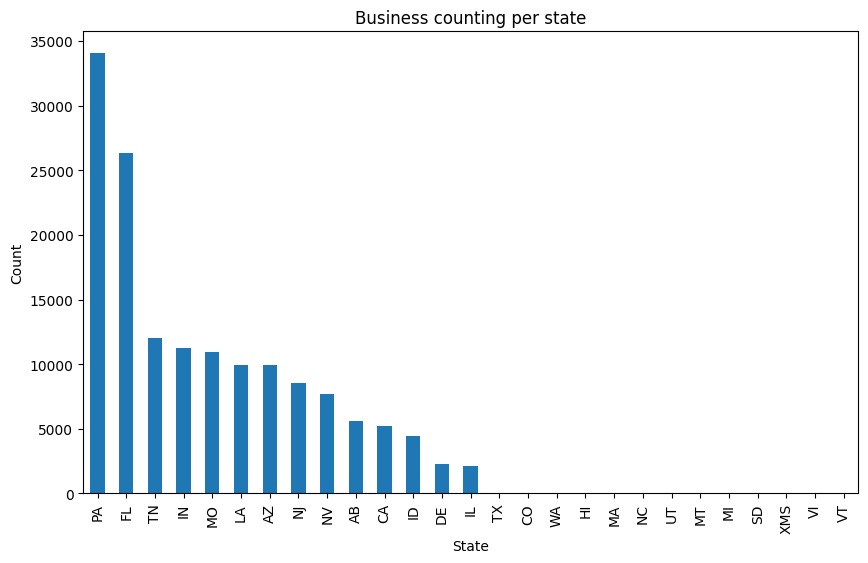
\includegraphics[scale=0.5]{../Images/dataexp.png}
\end{figure}
From the Figure \ref{fig:buscount} we can see that in "PA", we refer to Pennsylvania, a state located in the northeastern part of the United States. So I decided to conduct my analysis over the "PA" state due the amount of businesses present over there. Furthermore due the high dimension of the df it's difficult to create others type of graphics.
\section{Data Filtering}
As we discussed in the previous section \ref{sec:visdata} we want to targeting our recommender system in a specific area for a specific type of business. So I decided to take \textit{"PA"} as state and \textit{"Restaurant"} as type of business. Moreover I filtered the new dataframe called \texttt{restaurant\textunderscore df} with another parameter called \texttt{is\textunderscore open} that when is equal to 1 means that this business is actually a running business.
\begin{lstlisting}[language={Python},label={lst:filtdata},caption={Filtering Pyspark df}]
# Filtering data
restaurant_df = df_business_pandas[(df_business_pandas['state'] == state) & (df_business_pandas['is_open'] == 1) & df_business_pandas['categories'].str.contains(type_business)==True].reset_index()
\end{lstlisting}
Here an example of \texttt{restaurant\textunderscore df} printed:
\begin{table}[h]
\centering
\small
\resizebox{\textwidth}{!}{%
\begin{tabular}{llllllllll}
\hline
\multirow{2}{*}{index} & \multirow{2}{*}{address} & \multirow{2}{*}{attributes} & \multirow{2}{*}{business\_id} & \multirow{2}{*}{categories} & \multirow{2}{*}{city} & \multirow{2}{*}{is\_open} & \multirow{2}{*}{name} & \multirow{2}{*}{stars} & \multirow{2}{*}{state} \\
 & & & & & & & & & \\
\hline
3 & 935 Race St & (None, None, 'full\_bar', \{'touristy': False, '... & MTSW4McQd7CbVtyjqoe9mw & Restaurants, Food, Bubble Tea, Coffee \& Tea, B... & Philadelphia & 1 & St Honore Pastries & 4.0 & "PA" \\
\hline
\end{tabular}%
}
\caption{Example of a restaurant\_df's row}
\label{tab:rowrest}
\end{table}
Note that the attribute and category columns must be preprocessed before being used.
\section{Data preprocessing}
Lets start to analyze the attribute column. As we can see they are in this form:
\begin{lstlisting}[language={Python},label={lst:attritemex},caption={Attributes item example}]
Row(AcceptsInsurance=None, AgesAllowed=None, Alcohol="u'none'", Ambience=None, BYOB=None,..)
\end{lstlisting}
So we need a function that allow us to extract key-value pairs in a format understandable to Python. Here the snippet:
\begin{lstlisting}[language={Python},escapechar=|,label={lst:extractvalue},caption={Extracting key-value from attributes}]
# Function for extracting key-value from attributes
def extract_values(row):
    if row is None or row == "{}":
        return {}
    
    attributes = {}
    pattern = r"(\w+)\s*=\s*([^,]+)" |\label{line:re}|
    matches = re.findall(pattern, row)
    
    for key, value in matches:
        value = value.strip("'")
        attributes[key] = value
    
    return attributes
\end{lstlisting}
To achieve the result I used the regular expression. More specifically the line~\ref{line:re} defines a regular expression pattern.The pattern captures two groups:
\begin{itemize}
 \item the key (composed of one or more word characters \texttt{\textbackslash w$+$})
 \item the value (composed of one or more characters that are not a comma \texttt{\textbackslash $[\hat,]+$}), separated by an equal sign with optional whitespace around it.
 \end{itemize} 
Then we apply the function over all the rows of column attributes.
Now that the format seems to be good we proceed to create an entire \texttt{restaurant\textunderscore df\textunderscore attr} in which the attributes are extracted making a new column of the df and populating it with 0 or 1 based on their original value. An example are in the Table \ref{tab:restattrtable}.
\\
\begin{table}[]
\caption{Example of \texttt{restaurant\textunderscore df\textunderscore attr} elements} 
\label{tab:restattrtable}
\begin{tabular}{|l|l|l|l|l|l|}
\hline
BestNights & RestaurantsCounterService & WiFi & ... & Smoking & CoatCheck \\ \hline
0          & 1                         & 0    & ... & 0       & 0         \\ \hline
1          & 0                         & 1    & ... & 1       & 1         \\ \hline
\end{tabular}
\end{table}
We apply this reasoning also for categories obtaining the \texttt{df\textunderscore categories\textunderscore dm}. It will be useful to create the \texttt{df\textunderscore total}, a fundamental component for the recommender system. So in the Chapter \ref{ch:recsys} we are going to understand how recommendation systems work in theory.
\chapter{Recommender system}\label{ch:recsys}
As we mentioned in the Chapter \ref{ch:introduction}, there are two main basic architectures for a recommendation system. In my project I developed from scratch  more on a \textit{Content-Based} recommendation system. They are based on properties of items and the similarity of these are determined by measuring the similarity in their properties.
However I also worked with the ALS as \textit{Collaborative Filtering} using the PySpark library to compare mine with the one developed with the library. In this Chapter we give to the reader the general notion behind recommender system based on the reference book \cite{rajaraman2014mining}.
\section{Content-Based Recommendations}
We are starting to understand what is an item profiles. It's a record or collection of records representing important characteristics of the item. For example if we consider the restaurants as type of business of this project, we can say that the features of a restaurants can be all the attributes such as \textit{GoodForKids,BusinessAcceptsBitcoin,DogsAllowed...}.
In order to be a recommender system we need also the user. Indeed also the users has their profiles that describes their preferences. \par
Another fundamental aspect is the utility matrix. It's giving for each user-item pair, a value that represents what is known about the degree of preference of that user for that item. Without a utility matrix, it is almost impossible to recommend items. Usually there are two main approaches: 
\begin{itemize}
 \item We can ask users to evaluate items. We fall in this case because the from the dataset \texttt{review} we can access to all user-business pair reviews with the respective rate.
 \item We can make inferences from user's behavior. Indeed if one user buy something online or just watched a video we can say that he liked it.
 \end{itemize} 
Our ultimate goal for content-based recommendation is to create both a item profile consisting of feature-value pairs and a user profile summarizing the preferences of the user,based of their row of the utility matrix.If we consider profiles as vectors we can compute the cosine similarity in the space of the features and understand if the vectors appears closer or not. In this way we can recommend business to the user based on his preferences.
\section{Collaborative Filtering}
When we are referring to Collaborative Filtering we are focusing on the similarity of the user ratings for two items. In place of the item-profile vector for an item, we use its column in the utility matrix. User are similar if their vectors are close according to some notion of distance measures such as cosine distance. The process of identifying similar user and recommending what similar users like is called collaborative filtering.
\chapter{Creation of a Content-based Recommender system}\label{ch:recsyscontbased}
Before I talk about the content-based recommendation system that I created from scratch, I want to highlight some of the steps that allowed me to arrive at the solution or at least allowed me to learn more about the data I had at my disposal.
\section{Business similarity suggestion with Pandas and cosine similarity}\label{bussimpand}
First of all I tried to create a suggestion system by looking the business similarity. For achieve this goal I used in this step Pandas. I performed this steps:
\begin{enumerate}
\item Extract the reference restaurant index
\item Mapping the rate (1-3 stars will be mapped in 0 and 4-5 in 1)
\item Create the \texttt{cosine\textunderscore similarity\textunderscore scratch} function
\begin{lstlisting}[language={Python},escapechar=|,label={lst:cosinesim},caption={Cosine similarity function}]
def cosine_similarity_scratch(vector1, vector2):
    dot_product = np.dot(vector1, vector2)
    norm_vector1 = np.linalg.norm(vector1)
    norm_vector2 = np.linalg.norm(vector2)
    
    if norm_vector1 == 0 or norm_vector2 == 0:
        return 0.0
    
    similarity = dot_product / (norm_vector1 * norm_vector2)
    return similarity

\end{lstlisting}
\item Calculate business similarity respect the one selected. Order the similar restaurants in a descending way and then select n (= 5 in this case) top similar restaurant and print it.
\begin{lstlisting}[language={Python},escapechar=|,label={lst:simpandas},caption={Suggestion system in Pandas}]
restaurant_features = features_df.iloc[restaurant_index, 6:-2].values  # Reference restaurant feature vector

similarities = []
for i in range(len(features_df)):
    if i != restaurant_index:
        other_restaurant_features = features_df.iloc[i, 6:-2].values
        similarity = cosine_similarity_scratch(restaurant_features, other_restaurant_features)
        similarities.append(similarity)

similarities = np.array(similarities)
similar_restaurants = similarities.argsort()[::-1]  # Similar restaurant ordered in a desc way

# Visualize 5 top suggested restaurants with cosine sim column
top_similar_restaurants = similar_restaurants[:5]
recommended_restaurants = df_total.iloc[top_similar_restaurants][['name', 'stars']]
recommended_restaurants['cosine_similarity'] = similarities[top_similar_restaurants]

print(recommended_restaurants)

\end{lstlisting}
\end{enumerate}
So now I will show the results obtained.
\subsection{Experiment}
I choose the \texttt{8071} restaurant index called \texttt{Adelita Taqueria \& Restaurant}.
It's a mexican restaurant located in 1108 S 9th St Philadelphia, PA 19147. In the note the link of the restaurant on Yelp.\footnote{\url{https://www.yelp.com/biz/adelita-taqueria-and-restaurant-philadelphia?osq=Adelita+Taqueria\%26+Restaurant}}
The restaurant counts 39 reviews with an average rating of 4.5 stars.\par
The similar business that the system recommend are these reported in the Table \ref{simrespand} where there are linked their Yelp page.
\begin{table}[]
\caption{Top similar business recommended in Pandas}
\label{simrespand}
\begin{tabular}{|l|l|l|l|}
\hline
     & name                           & stars & cosine\_similarity \\ \hline
7109 & \href{https://www.yelp.com/biz/los-taquitos-de-puebla-philadelphia-4?osq=Los+Taquitos+de+Puebla}{Los Taquitos de Puebla}         & 4     & 1.000000           \\ \hline
5990 & \href{https://www.yelp.com/biz/san-antonio-mexican-cousine-hatfield?osq=San+Antonio+Mexican+cousine}{San Antonio Mexican cousine}    & 5     & 1.000000           \\ \hline
3534 & \href{https://www.yelp.com/biz/los-cuatro-soles-philadelphia?osq=Los+Cuatro+Soles}{Los Cuatro Soles}              & 5     & 0.942809           \\ \hline
3292 & \href{https://www.yelp.com/biz/ecowas-african-restaurant-philadelphia-2}{El Limon - Norristown}          & 4     & 0.942809           \\ \hline
1525 & \href{https://www.yelp.com/biz/la-hacienda-mexican-restaurant-bensalem?osq=La+Hacienda+Mexican+Restaurant}{La Hacienda Mexican Restaurant} & 4     & 0.942809           \\ \hline
\end{tabular}
\end{table}
They are all mexican restaurant so it's perfectly matching our selected restaurant.
I tried also to use a cosine similarity library from \texttt{from sklearn.metrics.pairwise import cosine\_similarity} and the results are quite similar as shown in Table \ref{simrespandsklearn}.
\begin{table}[]
\caption{Top similar business recommended in Pandas with sklearn cosine similarity}
\label{simrespandsklearn}
\begin{tabular}{|l|l|l|}
\hline
name                        & cosine similarity  & stars \\ \hline
San Antonio Mexican cousine & 0.9999999999999999 & 5     \\ \hline
Los Taquitos de Puebla      & 0.9486832980505138 & 4     \\ \hline
\href{https://www.yelp.com/biz/ecowas-african-restaurant-philadelphia-2}{El Charro Negro            } & 0.9486832980505138 & 4     \\ \hline
El Limon - Norristown       & 0.9128709291752769 & 4     \\ \hline
\href{https://www.yelp.com/biz/plaza-garibaldi-philadelphia-3?osq=Plaza+Garibaldi}{Plaza Garibaldi}             & 0.8999999999999999 & 4     \\ \hline
\end{tabular}
\end{table}
\section{Business similarity suggestion with k-NN algorithm}
I continued my search for similar restaurants also based on the k-nn algorithm. In brief it's a a supervised machine learning approach called k-nearest neighbors (k-NN) and it is utilized for both classification and regression problems. It is a non-parametric algorithm that bases its predictions on how closely new input data and training examples resemble each other. \par
The "k" in the k-NN method denotes how many nearest neighbors are taken into account while producing predictions.
The steps done are the following: 
\begin{itemize}
\item Take features excluding name and stars from the \texttt{df\_total} as x and stars as y
\item Splitting the data into training set and test set 
\item To figure out which k to choose, I applied 5-fold cross-validation and the best value for k is 20.
\item Then I fitted the model and printed the results \par
\texttt{Score on training set: 0.5624903205823137 ; Score on test set: 0.52198142486068}
\item Testing the model and use the last row as the validation test 
\item Getting the similar restaurants compared with the one taken in the validation test.
\end{itemize}
In the end, the results obtained are comparable with the other two approaches (cosine similarity from scratch and sklearn).
\section{Business similarity suggestion with PySpark and cosine similarity}
In this section I wanted to focus more on the scalability of the system. Therefore, I converted the approach used in section \ref{bussimpand} to PySpark, performing all the preprocessing by obtaining \texttt{df\_final\_spark}. Specifically, I summarize the operations:
\begin{itemize}
\item Transform the categories into a list of categories for the business
\item Perform filtering by state and business type.
\item Extract the attributes as columns and then having some columns of nested attributes I re-run the operation
\item Transform the values to 0-1 obtaining the \texttt{df\_business\_attr\_spark}
\item Same for categories creating the \texttt{df\_categories\_dm}
\item Finally I get the \texttt{df\_final\_spark} by the join between the categories,attributes and the \texttt{restaurant\_df\_sel\_spark} which contains the name and ratings of the various businesses.
\end{itemize}
Once I had completed all the preprocessing phase and obtained the various df's I could proceed with the recommendation. As seen in the code shown I created the \texttt{df\_matrix} that contains \textit{business\_id,features}. The features were generated using \texttt{VectorAssembler}.It is a feature transformer that combines multiple input columns into a single vector column.
\begin{lstlisting}[language={Python},escapechar=|,label={lst:simpyspark},caption={Suggestion system in PySpark}]
# Exclude the 'business_id' column from df_final
columns = [c for c in df_final_spark.columns if c != 'business_id']

# Convert binary values to integers
df_numeric = df_final_spark.select(['business_id'] + [col(c).cast('integer') for c in columns])

# Fill NaN values with 0
df_filled = df_numeric.fillna(0, subset=columns)

# Use VectorAssembler to create a feature vector column
assembler = VectorAssembler(inputCols=columns, outputCol='features')
df_matrix = assembler.transform(df_filled).select('business_id', 'features')
\end{lstlisting}
After that I proceeded to run the same test on the \textit{Adelita Taqueria \& Restaurant} using \texttt{cosine\_similarity\_spark} slightly modified to make it work properly with the PySpark pipeline.
In this case I wanted to select 15 as the number of recommendations.This is the table obtained:\par
\begin{table}[h]
\caption{Top similar business recommended in PySpark}
\begin{tabular}{|l|l|l|l|}
\hline
\multicolumn{1}{|c|}{business\_id}            & \multicolumn{1}{c|}{cosine\_similarity} & \multicolumn{1}{c|}{name}                        & \multicolumn{1}{c|}{stars} \\ \hline
\multicolumn{1}{|c|}{F2QwLwzS3vF9os0...} & \multicolumn{1}{c|}{{[}{[}1.0{]}{]}}    & \multicolumn{1}{c|}{San Antonio Mexican cousine} & \multicolumn{1}{c|}{4.5}   \\ \hline
DwOhLOd9Say...   & {[}{[}0.9803789354850793{]}{]} & Los Taquitos de Puebla & 3.5 \\ \hline
EoQiJ5D-pyWc...  & {[}{[}0.9714285714285714{]}{]} & El Primo Taqueria      & 4.5 \\ \hline
XQewVfTaosZ3U-4g...  & {[}{[}0.9714285714285714{]}{]} & Los Cuatro Soles       & 4.5 \\ \hline
mKJ\_WV7TvrjyDjm... & {[}{[}0.9710083124552245{]}{]} & El Limon - Bensalem    & 4.5 \\ \hline
SVf23pjKERkedqCdWl6ECA   & {[}{[}0.9660917830792959{]}{]} & Teresa's Mesa          & 4.0 \\ \hline
5ItgryJvadUrKVljjJ8l4g   & {[}{[}0.9660917830792959{]}{]} & Que Chula Es Puebla    & 4.0 \\ \hline
rNg75hKR0UIB5-jX5WiVQg   & {[}{[}0.9660917830792959{]}{]} & Los Mariachis          & 3.5 \\ \hline
1MVMKUvZfWwIqkhxP3rYvQ   & {[}{[}0.9613406389911041{]}{]} & Indian Garden          & 4.0 \\ \hline
sKUs4ISUgn3j6SeLYvSByg   & {[}{[}0.9613406389911041{]}{]} & El Charro Negro        & 4.0 \\ \hline
x1CtK2qnlCr\_1DJFNo1\_vw & {[}{[}0.9583148474999098{]}{]} & El Limon - Norristown  & 4.0 \\ \hline
venWfi69QVylbyrvaPt0nQ   & {[}{[}0.9578414886923188{]}{]} & Cafe Ynez              & 4.5 \\ \hline
t0Qyogb4x--K9i5b0AoDCg   & {[}{[}0.9578414886923188{]}{]} & Taco Maya              & 4.5 \\ \hline
fcAaBcYFo1YqetIjs9l8Iw   & {[}{[}0.9566222088265397{]}{]} & Sungate Diner          & 4.5 \\ \hline
uh-387pbyipzjCMcj5Dy6w   & {[}{[}0.9566222088265397{]}{]} & Las Palmas Del Sur     & 4.5 \\ \hline
\end{tabular}
\end{table}
Also you can see that they are all restaurants that cook Mexican style. But these methods are based solely and exclusively on the profile of the restaurants without taking into account the feedback that the user has given to the various restaurants. For this reason, I decided to continue the project by introducing the user profile component as well.
\section{Collaborative filtering with ALS ml library}
In collaborative filtering, matrix factorization is the state-of-the-art solution for sparse data problem, although it has become widely known since Netflix Prize Challenge.
A matrix factorization is a factorization of a matrix into a product of matrices. 
In the case of collaborative filtering, matrix factorization algorithms work by decomposing the user-item interaction matrix into the product of two lower dimensionality rectangular matrices.One matrix can be seen as the user matrix where rows represent users and columns are latent factors. The other matrix is the item matrix where rows are latent factors and columns represent items \cite{matrixfact}. Here's a picture that describe the matrix factorization.
\begin{figure}[hbtp]
\caption{Example of Matrix Factorization}
\centering
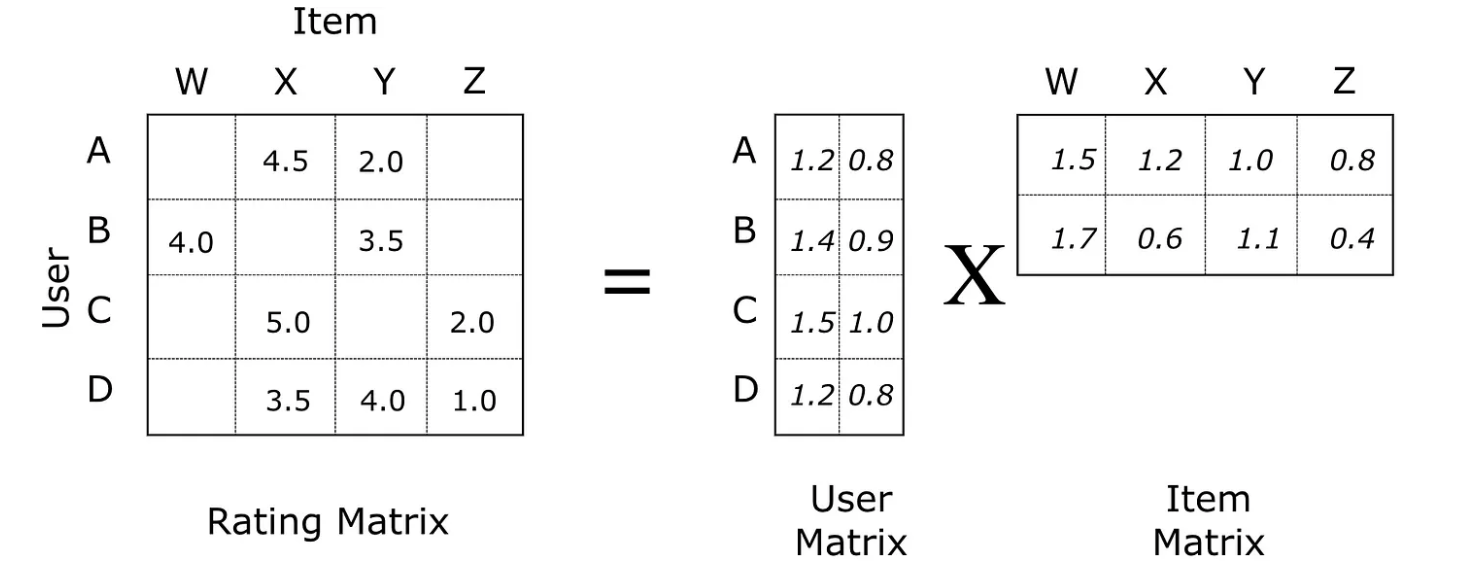
\includegraphics[scale=0.6]{../Images/matrixfact.png}
\end{figure}
The advantages of using this approach are mainly two:
\begin{itemize}
\item Model learns to factorize rating matrix into user and business representations, which allows model to predict better personalized business ratings for users
\item Less-known business can have rich latent representations as much as popular business have
\end{itemize}
More formally, in a sparse user-item interaction matrix the predicted rating user \textit{u} will give item \textit{i} is computed as:
$$r_{ui} = \sum_{f=0}^{nfactors} H_{u,f}W_{f,i}$$
Rating of item i given by user u can be expressed as a dot product of the user latent vector and the item latent vector.  Latent factors are the features in the lower dimension latent space projected from user-item interaction matrix.\par
Increasing the number of latent factors will improve personalization, until the number of factors becomes too high, at which point the model starts to overfit. A common strategy to avoid overfitting is to add regularization terms to the objective function.\par
The objective of matrix factorization is to minimize the error between true rating and predicted rating.
\subsection{Alternating Least Square (ALS) with Spark ML}
Alternating Least Squares (ALS) is a parallel matrix factorization algorithm. It is implemented in Apache Spark ML and specifically designed for large-scale collaborative filtering problems. ALS effectively addresses scalability and sparsity issues commonly encountered with Ratings data. Furthermore, ALS exhibits simplicity and demonstrates excellent scalability even when handling massive datasets. The main points are:
\begin{itemize}
\item ALS uses L2 regularization
\item ALS minimizes two loss functions alternatively; It first holds user matrix fixed and runs gradient descent with item matrix; then it holds item matrix fixed and runs gradient descent with user matrix
\item Its scalability: ALS runs its gradient descent in parallel across multiple partitions
\end{itemize}
So let's get to the heart of the matter by taking a look at the code.
Starting with \texttt{df\_review\_spark\_indexed} I go to convert the profile ids to numeric format using the \texttt{StringIndexer}. Once this is done we go to split the data into training set and test set as reported by this code:
\begin{lstlisting}[language={Python},escapechar=|,label={lst:splittraintest},caption={Splitting dataset in training and test set for ALS}]
(training, test) = df_review_spark_indexed.randomSplit([0.8, 0.2])
\end{lstlisting}
After that, the recommendation model based on the ALS model is created:
\begin{lstlisting}[language={Python},escapechar=|,label={lst:splittraintest},caption={Building recommended system model based on the ALS model}]
# Build the recommendation model using ALS on the training data
als = ALS(maxIter=5, regParam=0.01, userCol="user_id_index", itemCol="business_id_index", ratingCol="stars_review")
model = als.fit(training)
\end{lstlisting}
There are some parameters that need to be considered such as:
\begin{itemize}
\item \texttt{maxIter}: is the maximum number of iterations to run
\item \texttt{regParam}: specifies the regularization parameter in ALS
\item \texttt{userCol}: as suggested from the name is the column of the user 
\item \texttt{itemCol}: as suggested from the name is the column of the item 
\item \texttt{ratingCol}: as suggested from the name is the column of the rating 
\end{itemize}
This operation requires times according to the type of technical specifications you have. Those used in the project are specified in the section \ref{sec:sysspec}.
Once we have fitted the model with the training data we can proceed to test our model with the test set.
\begin{lstlisting}[language={Python},escapechar=|,label={lst:predals},caption={Prediction over the test set with the ALS model}]
predictions = model.transform(test)
#predictions.show()
\end{lstlisting}
Then I proceeded to test the model by filtering for a generic user id which in this case is \texttt{user\_id\index = 14269.0} by descendingly sorting the prediction column. \par
To then understand the goodness-of-fit of the model, I calculated the NDCG (see the section \ref{sec:ndcg}) by manipulating the df columns as can be seen from the code:
\begin{lstlisting}[language={Python},escapechar=|,label={lst:ndcgals},caption={Calculating the ndcg over the predictions df obatined in ALS}]
from pyspark.sql.functions import expr

predictions = predictions.withColumn("rank", expr("row_number() over (partition by user_id_index order by prediction desc)"))
predictions = predictions.withColumn("dcg", expr("1 / (log2(rank + 1))"))
predictions = predictions.withColumn("idcg", expr("1 / (log2(1 + rank))"))
ndcg = (
    predictions
    .groupBy("user_id_index")
    .agg(expr("sum(dcg) as dcg_sum"), expr("sum(idcg) as idcg_sum"))
    .select(expr("avg(dcg_sum / idcg_sum)").alias("ndcg"))
    .collect()[0][0]
)
\end{lstlisting}
Printing the metric we get \texttt{ndcg = 1.0}. A value of NDCG of 1 indicates that the system has produced perfect recommendations corresponding to user preferences.
\section{Content based recommendation from scratch in PySpark}

\chapter{Scalability and complexity}\label{ch:scalability}
\section{System specification}\label{sec:sysspec}
\chapter{Results and experiments}\label{ch:results}
\section{NDCG}\label{sec:ndcg}
\chapter{Conclusion}\label{ch:conclusion}
%dataset reduced


\lstlistoflistings
\bibliographystyle{unsrt}
\bibliography{biblio}
\end{document}
